% !TeX root = RJwrapper.tex
\title{RTCGA.methylation Explorator documentation}
\author{by Katarzyna Sobiczewska}

\maketitle


\section{Introduction}\label{introduction}

The RTCGA package \citep{kb} provides accessible and easy way to analyse
data from TCGA project (visit this page:
\href{http://cancergenome.nih.gov/}{\url{http://cancergenome.nih.gov/}}
to get more information about the project).

The RTCGA.methylation Explorator allows you to go into the data (source:
\href{https://github.com/RTCGA/RTCGA.methylation}{\url{https://github.com/RTCGA/RTCGA.methylation}}
) and visualize interesting connections between DNA characteristics and
the length of survival time of patiens stricken with different types of
cancer.

\section{Data specifications}\label{data-specifications}

The application allows you to explore 9 different types of cancer which
are collected in different datasets with number of observations given in
braces:

\begin{itemize}
\itemsep1pt\parskip0pt\parsep0pt
\item
  Breast invasive carcinoma - BRCA (343)
\item
  Colon adenocarcinoma - COAD (202)
\item
  Glioblastioma multiforme - GBM (283)
\item
  Pan-kidney cohort - KIPAN (973)
\item
  Kidney renal clear cell carcinoma - KIRC (439)
\item
  Acute Myeloid Leukemia - LAML (194)
\item
  Lung adenocarcinoma - LUAD (89)
\item
  Lung squamous cell carcinoma - LUSC (160)
\item
  Uterine Corpus Endometrial Carcinoma - UCEC (118)
\end{itemize}

For each observation we had almost \textbf{300,000 features} which were
expressed by different loci on DNA. Data values are from unit interval
and they describe percentage of methylation for each biomarker.

To select the most important biomarkers the RTCGA.methylation dataset
was merged with clinical information about each patient and time of
survival was used to extract features which are significant. Using
\textbf{Kaplan-Meier's estimator} we compared times of survival in
strata indicated by median of methylation value. A biomarker was
important if the differenece for survival was signifiant, thus almost
300,000 tests was made (more informaction about used methods you can
find here \citep{kmsurvdiff}).

In this way we extracted over \textbf{13,000 biomarkers} that are
significant for survival. They are listed in \texttt{Gene names} panel.

\section{Application details}\label{application-details}

The main goal of this application is to visualize survival influences in
time for given biomarkers. Insight into distribution of biomarkers is
also provided. The application has three main panels:

\subsubsection{1. Survival}\label{survival}

Here you can inquire the influence of particular biomarkers on survival
and differences between them in different types of cancer. The
Kaplan-Meier methods was used \citep{km}.

\subparagraph{Output details}\label{output-details}

\begin{itemize}
\itemsep1pt\parskip0pt\parsep0pt
\item
  \textbf{Survival curves} with possibility to customise strata by
  setting up methylation cut-off.
\item
  \textbf{Significance level} (p-value) for given biomarker that has an
  influence on survival in strata indicated \textbf{by median}.
\item
  \textbf{Odds ratio} for time interval and startum set up by user.
  Note, that there is no possibility to calculate odds ratio with single
  stratum. In that case change the methylation cut-off so as to obtain
  two groups to compare with each other. If you are not sure about
  appropriate threshold value, take advantage of
  \texttt{Biomarkers distribution} panel.
\end{itemize}

\subsubsection{2. Biomarkers
distribution}\label{biomarkers-distribution}

In this place you can find what is the distribution of methylation
values for the biomarkers in different types of cancer. Are there any
similarities between them?

\subparagraph{Output details}\label{output-details-1}

\begin{itemize}
\itemsep1pt\parskip0pt\parsep0pt
\item
  \textbf{Boxplots} and \textbf{density plots} for each biomarker.
\item
  \textbf{Kolmogorow-Smirnov test} results from comparing a biomarker
  distribution in each two types of cancer. One-sided test was used in
  this place and the results are gathered as a table. You can choose if
  you want to see results as p-values or decisions (one from
  ``\textless{}'', ``=''). Decision are made with \(\alpha=0.05\).
  Distributions are recognized as equal if we have decision: ``='' on
  both sides of diagonal.
\end{itemize}

On the following example we can observe some similarities in
distribution between cancer types, however Kolmogorov-Smirnov test:

H0: cancer=CANCER

H1: cancer\textless{}CANCER

reveal that only KIRC and KIPAN distributions of \texttt{cg14226064} are
the same (KIRC=KIPAN vs KIRC\textless{}KIPAN hypothesis was accepted as
well as KIPAN=KIRC vs KIPAN\textless{}KIRC).

\begin{figure}[htbp]
  \centering
  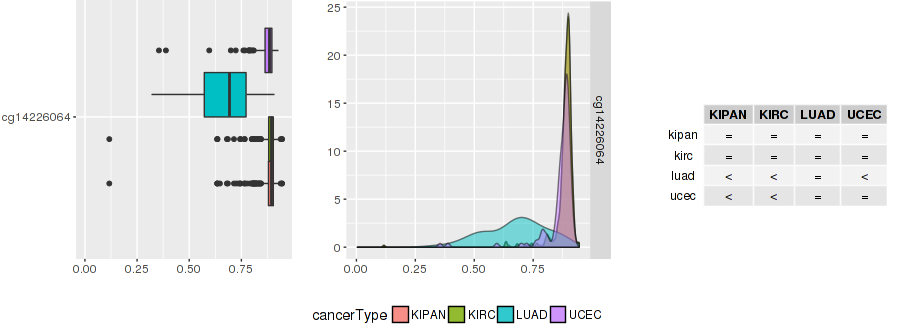
\includegraphics[scale=0.45]{kstest}
  \caption{Biomarkers distribution example}
  \label{figure:rlogo}
\end{figure}

\subsubsection{3. Biomarkers list}\label{biomarkers-list}

If gene names is more preferable way for you to explore this data,
please use the \texttt{Biomarkers list} panel to find biomarkers that
are suitable to your genes list.

\subparagraph{Output details}\label{output-details-2}

\begin{itemize}
\itemsep1pt\parskip0pt\parsep0pt
\item
  \textbf{Biomarker name} - names used in this application.
\item
  \textbf{Gene name} (in accordance with given locus). Notice, that one
  locus may have more than one accordant gene as well as one gene may
  have more than one suitable loci.
\item
  \textbf{Common for (w/ p.val for survival)} - here the p-value is the
  measure of biomarker significancy for survival where strata are
  defined by median.
\item
  \textbf{Number of common cancers} - number of cancer types for which a
  biomarker is significant for survival.
\end{itemize}

\subsection{Additional tips}\label{additional-tips}

The application gives you possibility to download results and modify on
your computer. The table is write as csv file. Plot outputs are saving
as \texttt{ggplot} objects and they might be modify only with
\texttt{ggplot2} R package.

\bibliography{RJreferences}

\address{%
Katarzyna Sobiczewska\\
\\
\\
}
\href{mailto:fk.katarzyna@gmail.com}{\nolinkurl{fk.katarzyna@gmail.com}}

